
\documentclass[12pt]{report}
\usepackage{textcomp}

\addtolength{\hoffset}{-2.25cm}
\addtolength{\textwidth}{4.5cm}
\addtolength{\voffset}{-2.5cm}
\addtolength{\textheight}{5cm}
\setlength{\parskip}{0pt}
\setlength{\parindent}{15pt}

\usepackage{graphicx}
\graphicspath{ {./images/} }

\pagestyle{plain}

\usepackage{amsthm}
\usepackage{amsmath}
\usepackage{amssymb}

\usepackage[colorlinks = true, linkcolor = black, citecolor = black, final]{hyperref}

\usepackage{graphicx}
\usepackage{multicol}
\usepackage{ marvosym }
\usepackage{wasysym}

\usepackage{outlines}
\usepackage[utf8]{inputenc}
\usepackage[english]{babel}

\usepackage{enumitem,amssymb}
\newlist{todolist}{itemize}{2}
\setlist[todolist]{label=$\square$}
\usepackage{pifont}
\newcommand{\cmark}{\ding{51}}%
\newcommand{\xmark}{\ding{55}}%
\newcommand{\done}{\rlap{$\square$}{\raisebox{2pt}{\large\hspace{1pt}\cmark}}%
\hspace{-2.5pt}}
\newcommand{\wontfix}{\rlap{$\square$}{\large\hspace{1pt}\xmark}}

\newcommand{\pr}[1]{\left(#1\right)}

\usepackage{xcolor}
\definecolor{forestgreen}{RGB}{1, 97, 89}
\definecolor{green}{RGB}{0, 150, 0}
\definecolor{yellow}{RGB}{218, 165, 32}

\usepackage{pgfplots}
\pgfplotsset{compat=1.16}
\usepackage{circuitikz}
\usepackage{tikz}
\usetikzlibrary{patterns}
\usetikzlibrary{arrows.meta}

\setlength{\parindent}{0in}

\pagestyle{plain}

\begin{document}

\bigskip
\bigskip
\bigskip
\bigskip
\begin{titlepage}

   \begin{center}
       \vspace*{2in}

       \textbf{\Huge Forcing a meaninful future: \\ Brain-spine-muscle interfaces\\
       \smallskip }

       \vspace{0.5in}

       \textbf{\large By Jackson Powell \\ \small For future Jackson}

    \vspace{1cm}

    \begin{center}
        Once you know the way broadly, you can see it in all things.\\
        -- The Book of Five Rings by Miyamoto Musashi
    
    \end{center}


\vspace{0.5cm}
        
\centerline{\rule{13cm}{0.4pt}}
\tableofcontents
\centerline{\rule{13cm}{0.4pt}}
            
       \vspace{0.8cm}
     
       \end{center}


\end{titlepage}

\pagebreak




{\scshape J. Powell} \hfill {\scshape \large Brain-spine-muscle} \hfill {\scshape Summer, 2023}
 
\smallskip

\hrule
\bigskip
\normalsize 



\section{Overview}

\subsection{Purpose}
The purpose of this book is to aggregate all of the content and tools I will need in forging the future I desire: building better brain-spine-muscle interfaces. 

\subsection{Content}
It is true that total recovery from spinal cord injury, in sever cases, will require both therapeutic and electronic intervention. One must therefore learn of physiology and electronics to be able to solve these problems.  

\vfill\pagebreak

\part[Electronics]{Electronics
            \vspace{0.2in}
            \begin{center}
            \begin{minipage}[l]{10cm}\small
                Like many of the vagabonds who live in the fields, stray horses seemed to him to be good-natured things. When you're through with them, they ask for nothing; they just go off quietly somewhere by themselves. \newline
                -- Musashi by Eiji Yoshikawa
            \end{minipage}
            \end{center}}

\chapter{Background Information} 

\section{How Electricity Works} 
\subsection{The misconception} One often represents electricity with the canonical metaphor of water flowing in a tube, equating the flow of water, which powers a wheel of some sort, as being the equivalent of electrons pushing through a wire. Incidentally, this simplifying schema illustrates a key misconception in the nature of electricity. This is easiest exemplified in the mode with which electricity reaches one's house from a power-plant, which before arriving will be subject to breaks in the circuit (transformers). In the traditional viewing of electricity, that which one is taught in early education, this is disconcerting as one would think that if electrons can not physically go from battery to bulb, then how can their kinetic energy be transferred and light it?\newline

When a battery sits without wires attached, around it is an electric field. This field does not dissipate because no electrons flow from it. When wires are attached, charge accumulates on the surface of the wires. This causes a small electric field within the wires, but the drift velocity of electrons within the wire is quite slow---nowhere near the speed of light. However, the flow of electrons within the wire is sufficient to drive an electric field which exists around the wires. From this, we can determine the direction that energy will flow by taking the cross product of the electric and magnetic fields. In fact, if an lightbulb is attached, this means that energy flows from the battery to the bulb in all directions, not through the wires itself.\newline 

Let us consider now what will happen with an AC circuit, where the electromotive force flips with each cycle. In this case, both the electric and magnetic fields switch directions, meaning that their cross product will remain the same and power the lightbulb. Notably, the electrons do not move much (if at all) in this setup---but this is not a surprise, as it is not the electrons that carry the energy anyway. Now, it is still essential to recognize that it is the movement of electrons within the filament of a lightbulb that creates light. This is, indeed, from kinetic energy transferred from electrons bouncing against the metals lattice, dissipating energy in the form of light. The necessary distinction is that it is not electrons that flow all the way from the battery, but rather it is vibrations of those that were, and always will be, within the bulb itself. When you consider it like this, it is straightforward---as the electric field derived from the battery is what provides the electrons with enough kinetic energy to power the bulb.\newline

Interestingly, comparisons to the ``water flow" model fail dramatically in the traditional sense, but the Venturi Effect used to describe fluid flow actually succeeds. In adding a bulb you add a resistor, which is comparable to adding a part of a pipe with a smaller diameter. As water will flow faster in this section of the tube, so too will electrons. In order to maintain the same current as is through the rest of the tube, the drift velocity, $\mathrm{V_d}$, must be higher. $\mathrm{V_d}$ is proportional to the electromotive force, E, meaning the force is highest within the bulb.\newline 

Of course you may say: ``well then why do we use wires at all?" The answer is that wires are helpful in channeling the fields, thereby making them more efficient. Knowing all of this, in this work I will almost invariable describe the flow of current as electrons moving through a wire. This is because it is much easier to think of electricity in this way, hence the ubiquitous misconception. 

\subsection{Nuances in the fields} It is worth explicitly highlighting that the electric field that causes the actual flow is from charges along the wires, rather than the battery. This is notable because if this were not the case, the proximity of the bulb to the battery would dictate its brightness. One may wonder how this type of charge distribution can be established so rapidly, and the reason is that the distance an electron needs to travel in order to create such a distribution is subatomic in size---meaning that with movement at the speed of light, the time it takes to establish a surface charge is effectively zero.\newline

The whole idea is quite unintuitive, so it is appropriate to keep it smushed in the back of your mind, and to only draw it out when encountering things that are otherwise strange---such as wireless charging, which should now be much more comprehensible. 



\section{Laws and Devices} The currents flowing in and out of a node will always be equal. The sum of the voltages over an entire circuit will always be equal. Kirchoff's Voltage Law (KVL) can be used to show that wires connected in parallel will have the same voltage across them. In this way, we can predict the current flowing through a circuit to be $\mathrm{V} = \mathrm{IR}$. The formula for power is given as: $\mathrm{VI} = \mathrm{P}$, which means that when one solves for voltage, and knowing that current is in units of charge/time and power in work/time, voltage is work per unit charge.\newline

Voltage is measured using a voltmeter, a device in parallel with the load you are interested in measuring. An ammeter is used to measure current, which will be in series with the current you are trying to measure. This means that the voltmeter should have an extremely high resistance, so as to not draw any current, and an ammeter to have a low resistance, so as to not have any voltage drop. These are important considerations, as if the resistance of the load you are measuring is large (say, $1\mathrm{M}\Omega$), it is possible that the voltmeter will have some non-negligible current flow through it. The same goes for if your circuit has very low resistance and you use an ammeter. To illustrate, one would measure the voltage and current coming from a battery as seen below:

\begin{center}
\begin{circuitikz}
\draw 
(0,2) to [battery, l=$\mathrm{V}_{s}$] (0,0)
(-2,0) to [voltmeter] (-2,2)
(-2,0) -- (0,0)
(-2,2) -- (0,2)
(0,2) to [ammeter] (3,2)
(3,2) to [R] (3,0)
(3,0) -- (0,0);
\end{circuitikz}
\end{center}

\subsection{Thevenin and Ideality} A Thevenin Circuit simplifies the circuit to have a single resistance, $\mathrm{R}_{th}$, and a single voltage, $\mathrm{V}_{th}$. $\mathrm{R}_{th}$ can be calculated via replacing all of the voltage sources with a wire, and disconnecting all of the current sources. This ``short circuits" your circuit and leaves you with only resistors, which can be used to calculate R$_{th}$ using the familiar resistor rules. One can also short circuit the terminals, and determine the current flow, giving us R$_{th} = \mathrm{V}_{th}/\mathrm{I}_{sc}$.\newline

R$_{th}$ can be measured in a circuit by varying the R$_{load}$ added to a circuit. In this case, you will see the voltage supplied (and corresponding current) change. The slope of this change $(\Delta \mathrm{V} / \Delta \mathrm{I})$ will equal R$_{th}$. If you vary the load through the two terminals and measure the voltage across it, you will get a graph that looks something like this:\newline  

\begin{center}
\begin{tikzpicture}
\begin{axis}[
    xlabel=$I_{out}$,
    ylabel=$V_{out}$,
    xmin=0, xmax=30,
    ymin=0, ymax=100,
    xtick={0},
    ytick={0}
            ]
\addplot[smooth,mark=*,color=red]
    plot coordinates {
        (15,0)
        (7.5, 45)
        (0,90)
    };
    \draw (3,90) node {$V_{oc}$};
    \draw (15,10) node {$I_{sc}$};
\end{axis}
\end{tikzpicture}
\end{center}

Again, the slope is what gives you R$_{th}$. I$_{sc}$ is an important value which allows you to calculate V$_{th}$. The current that flows when you short circuit the load (I$_{sc}$), multiplied by R$_{th}$, gives you V$_{th}$. 

\begin{multicols}{2}
\begin{center}
\begin{circuitikz}
\draw 
(1,2) to [R, l=$2k\Omega$] (1,0)
(-2,2) to [battery, l=$10V$] (-2,0)
(-2,0) -- (0,0)
(1,2) to [short, -*] (3,2)
(-2,2) to [R, l=$1k\Omega$] (1,2)
(3,0) to [short, *-] (0,0);
\end{circuitikz}
\end{center}

\begin{center}

\begin{circuitikz}
\draw 
(0,2) to [battery, l=$6.67V$] (0,0)
(0,2) to [R, l=$667\Omega$,-*] (3,2)
(3,0) to [short, *-] (0,0);
\end{circuitikz}
\end{center}
\end{multicols}

\subsubsection{The ideality of sources.}
This coaxes us lightly into the topic of source ideality. Imagine all voltage or current sources as having a resistor in parallel with it, but inside of the component itself. An ideal battery, or voltage source, would be able to drive the same voltage, irrespective of the resistor/current. This would be like having a battery whose internal resistance is 0, causing the entirety of the voltage drop to occur on the circuit fragments outside of the battery. In the real world, batteries are not ideal. The canonical illustration of a batteries ideality is in trying to use a 9V battery to start your car. Naturally, the voltage dwindles as the current supplied increases. You can calculate the internal resistance of a battery by adding increasingly large loads to it, thereby giving you the batteries IV curve. It is worth considering this, as if your R$_{load}$ is only $\approx 10 \times$ R$_{th}$, then you may see drooping in the voltage supplied. Another way to state this is to make sure that the \textit{input resistance} of your voltage source is much smaller than the \textit{output resistance} of the upcoming circuit fragment you are attempting to drive. \newline

This contrasts to a current source, whose desired internal resistance is $\infty$, as you will want no current to flow through it, and to flow entirely through the circuit fragments outside of the component. Once again, as the real world is not ideal, your goal in this case will be to have downstream circuit components whose input resistance is much smaller than the components output resistance.\newline

Building this kind of circuit only works when the IV curve of the circuit is linear. When isn't it?

\subsection{LED Circuits and PNP}

The IV curve across a light emitting diode (LED) should look something like this: 

\begin{centering}

\begin{tikzpicture}
\begin{axis}[
    xlabel=voltage (V),
    ylabel=current (mA),
    xmin=0, xmax=2.5,
    ymin=0, ymax=50,
    xtick={0, 0.5,...,2.5},
   % <---
    ytick={0, 10,...,50}
            ]
% can add points by inserting ,mark=* into the specifications
\addplot[smooth,color=red]
    plot coordinates {
(1, 0) 
(1.63, 1.5)
(1.72, 2) 
(1.77, 4)
(1.81, 6)
(1.86, 8)
(1.87, 10)
(1.89, 12)
(1.91, 14)
(1.93, 16)
(1.94, 18)
(1.96, 20)
(1.97, 30)
(1.98, 40)
(1.985, 50)
    };
\end{axis}
    \end{tikzpicture}
    
\end{centering}


The IV curve for a diode, like an LED, is exponential in that the current slowly increases after the voltage across a diode hits some ``threshold," after which the current rises exponentially with voltage. Why is this the case? A diode is a P-N junction bridged by some depletion zone. The P side of the diode contains positively charged elements that act as ``holes" (a silly way to say there is an absent electron position). The N side contains elements whose outer layers are loosely filled with electrons (i.e., low ionization energy). Effectively, the P side is devoid of electrons, while the N side has many free to give. What does this mean with regard to current and voltage? It means that the ``depletion zone" between the two requires electrons to be able to bridge the gap. This really can't happen unless they have a certain amount of energy, so increasing the voltage helps reach the ``threshold" energy requires to pass the depletion zone (think of P $=$ IV). Thus, as the electrons somewhat saturate the diode, you can theoretically pass an infinite current through it, as it will be effectively a short circuit. 



%%%%%%%%%%%%%%%%%%%%%%%%%%%%%%%%%%%%%%%%%%%%%%%%%%%%%%%%

\vfill\pagebreak
\part[Math and Models]{Math and Models
            \vspace{0.2in}
            \begin{center}
            \begin{minipage}[l]{10cm}\small
            \centering
                All truly strong people are kind. \newline
                -- Vagabond by Takehiko Inoue
            \end{minipage}
            \end{center}}

\chapter{Moving Through States}
\subsection{Markov-chains} Markov chains are useful in predicting the next state desired. 

\begin{center}
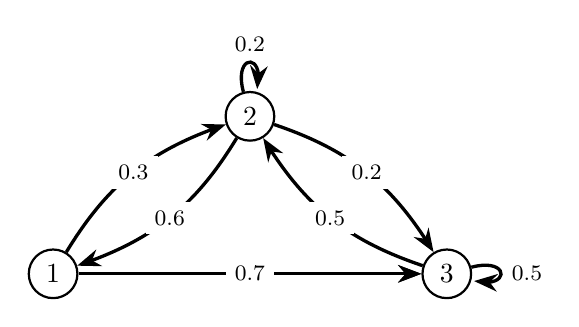
\begin{tikzpicture}
\begin{scope}[every node/.style={circle,thick,draw}]
    \node (A) at (0,0) {1};
    \node (B) at (2.5,2) {2};
    \node (C) at (5,0) {3};

    \end{scope}

\begin{scope}[>={Stealth[black]},
              every node/.style={fill=white,rectangle},
              every edge/.style={draw=black,very thick}]
    \path [->] (A) edge [bend left=20] node[pos=0.5] {\footnotesize{0.3}} (B);
    \path [->] (B) edge [bend left=20] node[pos=0.5] {\footnotesize{0.6}} (A);
    \path [->] (B) edge [bend left=20] node[pos=0.5] {\footnotesize{0.2}} (C);
    \path [->] (C) edge [bend left=20] node[pos=0.5] {\footnotesize{0.5}} (B);
    \path [->] (A) edge (C);
    \path [->] (A) edge node[pos=0.5] {\footnotesize{0.7}} (C);
    \path[<->] (C) edge [loop right] node {\footnotesize{0.5}} ();
    \path[<->] (B) edge [loop above] node {\footnotesize{0.2}} ();
    
    \end{scope}

\end{tikzpicture}
\end{center}


% \begin{equation} \label{eq8}
% \begin{split}
% N_{open1}^{i+1} &=  e^{-\Delta t / \tau_{open}}N_{open1}^{i} + \pr{1 - e^{-\Delta t P_{total}}}N_{closed}^{i} \\ 
% N_{open2}^{i+1} &= \pr{1 - e^{-\Delta t P_{total}}}N_{open2}^{i} + P_{P}\pr{1-e^{-\Delta t / \tau_{open}}}N_{open1}^{i} \\ 
% N_{inactive}^{i+1} &= e^{-\Delta t / \tau_{inact}}N_{inactive}^{i} + \pr{1-P_{P}}\pr{1-e^{-\Delta t / \tau_{open}}}N_{open1}^{i} + e^{-\Delta t P_{P}}N_{open2}^{i}\\
% N_{closed}^{i+1} &= e^{-\Delta t P_{total}}N_{closed}^{i} + \pr{1-e^{\Delta t / \tau_{inact}}}N_{inactive}^{i} \\
% \end{split}
% \end{equation}


Transition matrix: 
\begin{align}
\mathrm{A} =
\begin{bmatrix} %%%%%%%%%%%%%%
0           &  0.3          & 0.7 \\ 
0.6         &  0.2          & 0.2     \\
0           &   0.5         & 0.5    \\ 
\end{bmatrix}
\end{align}

\vfill\pagebreak
\part[Physiology]{Physiology
            \vspace{0.2in}
            \begin{center}
            \begin{minipage}[l]{10cm}\small
                ?? \newline
                -- ??
            \end{minipage}
            \end{center}}

\section{Central Pattern Generation}

Defining the central pattern generator is still somewhat contested. Computational models have been used to explore its existence\footnote{\url{https://www.nature.com/articles/s41598-021-91714-1}}, and for now we should take a few unifying assumptions: \textbf{(1)} the central pattern generator exists and is used to generate rhythmic moving, such as walking, \textbf{(2)} in many cases it is initiated by the CNS, but aside from that is largely devoid from CNS input, and \textbf{(3)} the CNS can work in tandem to compute integrated moving that requires coordination and balance. 



\part[Brain-Spine-Muscle Interfaces]{Brain-Spine Interfaces
            \vspace{0.2in}
            \begin{center}
            \begin{minipage}[l]{10cm}\small
                ??
                -- ??
            \end{minipage}
            \end{center}}

\chapter{Biochemistry}
\section{Therapeutic Approaches} While one may find it odd to begin an electronics discussion with a chapter on biochemistry, the fact of the matter is an integrated approach is the only way. 



\section{Historical Dealings}

Using electronics to study neural circuits has a long and storied history. One can think of Hodgkin and Huxley, whose ubiquitous nature avoids a need for citation, using an operational amplifier to clamp the voltage of giant squid axons to learn of their properties. In the case of solve spinal cord circuits, so too have electronics long been used\footnote{\url{https://journals.physiology.org/doi/epdf/10.1152/jn.1943.6.2.111}}.\newline

Restoration of the signals which pervade severance in spinal cord injury through therapeutics has been equally explored. For example, drugs such as clonidine, $\alpha_2$ receptor agonist, can promote walking in cats with spinal cord injury\footnote{\url{https://journals.physiology.org/doi/full/10.1152/jn.1998.79.6.2941}}. This effect can be blockedc completely by yohimbine, an $\alpha_2$ receptor antagonist\footnote{\url{https://www.ncbi.nlm.nih.gov/pmc/articles/PMC2278596}}.\newline

The ability to generate walking-like movements from electrical stimulation of the lower spine, the T10-L1 region, has been long known\footnote{\url{https://www.sciencedirect.com/science/article/pii/B9780444521378000188}}$^,$\footnote{\url{https://journals.sagepub.com/doi/pdf/10.1177/1073858417699790}}. In these instances, ``tonic" stimulation was able to generate step-like movements. Although the term ``tonic" is dubious because other papers by the same lab identified frequency dependence in their stimulation\footnote{\url{https://link.springer.com/article/10.1007/s00422-004-0511-5}}. While one can generate step-like movements at once frequency, continued extension can be generated with another. 


\section{Lorach, ..., Courtine 2023, Nature} This is the most recent iteration of an ongoing project by the Courtine group. It features a brain-spine interface (herein called BSI). 

\subsection{Overview} The group used surgical implantation into th skull, over the motor cortex, to record patient movements and wirelessly transmit this to the spinal cord. The technology used to capture these electrocorticographic (ECoG) signals is the WIMAGINE electrode array--- which features 64 electrodes on either side ($8 \times 8$ grid)\footnote{This seems like strikingly low resolution}. The design features two antennas, and the second of which transmits motor signals that are to be decoded and sent to a pulse generator. The pulse generator is ACTIVA RC, the same that is used in deep brain stimulation (DBS). 

\subsection{Shortcomings} The three shortcomings explicitly mentioned in the \textbf{Introduction} are that \textbf{(1)} one using this BSI must have motion sensors on in order to compensate (a sort of PID controller, perhaps),  \textbf{(2)} that the patient's movement was not perceived as natural, and \textbf{(3)} that there was still considerable hurdles in traversing variable terrain. Many more shortcomings exist than this, and we will go through them below.\newline

\subsubsection{Motion Sensors} I suppose it is obvious why one would use a motion sensor rather than an EMG---as it would be too difficult to discern whether the motion itself, or strength of contraction, is too high using an EMG alone. Still, though, I wonder if this is a feasible alternative. Perhaps one can simply predict motion based on EMG patterns.\newline

The largest drawback, in my opinion, is their desire to make it quickly programmed/calibrated. As with DBS, one would actually prefer longer calibration time. That is, one would be happy to wait a few extra hours or days if it makes their ability to walk improve.\newline

Similarly, they commented that the patient tested was able to walk without the BSI turned on (using crutches) after some time. This signals three things to me, \textbf{(1)} this patient's injury was not, per se, insurmountably severe, \textbf{(2)} the plastic abilities of a damaged spinal cord may be better than we had thought---especially since the patient's injury predated this treatment by 10 years, \textbf{(3)} that there was likely some important tuning being done by the brain-spine endogenous connection (i.e., their BSI was not doing all of the work), and \textbf{(4)} in some cases, no BSI is likely needed at all, and electrical stimulation may be sufficient. This in itself is a quite interesting, alternative patient state. For example, one can imagine a scenario where a patient's brain-spine communication is deeply dampened, but not entirely ceased by damage. Therefore, one would only need amplification of signals as opposed to complete generation of new ones. There may be some of that here. Another comment to make is that their signals are incredibly un-sophisticated, as presented in this paper. That is, they use 16 random electrodes, which do not have connections to synapses themselves. Perhaps this design is to hijack a more reflex-based approach to walking---hence why one can not traverse variable terrain that goes beyond reflexive movement.\newline

A comment regarding the surgery itself: The patient's are having two large, 50mm arrays placed into their skull. Naturally, most would agree to this in order to restore their ability to walk. However, it surprises me that they chose to make the device wireless, given that the surgery is already quite invasive. 

\subsubsection{Seven States} 

\begin{center}
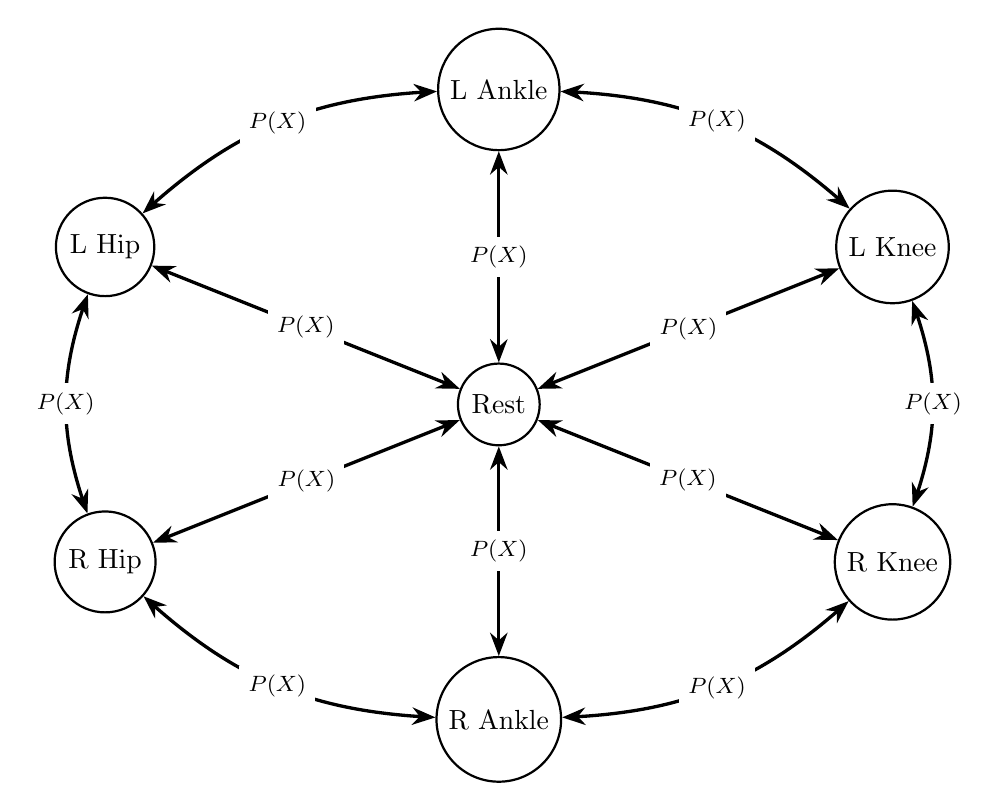
\begin{tikzpicture}
\begin{scope}[every node/.style={circle,thick,draw}]
    \node (Rest) at (0,0) {Rest};
    \node (LeftAnkle) at (0,4) {L Ankle};
    \node (LeftHip) at (-5,2) {L Hip};
    \node (LeftKnee) at (5,2) {L Knee};
    \node (RightAnkle) at (0,-4) {R Ankle};
    \node (RightHip) at (-5,-2) {R Hip};
    \node (RightKnee) at (5,-2) {R Knee};
    \end{scope}

\begin{scope}[>={Stealth[black]},
              every node/.style={fill=white,rectangle},
              every edge/.style={draw=black,very thick}]
    \path [<->] (Rest) edge node[pos=0.5] {\footnotesize{$P(X)$}} (LeftAnkle);
    \path [<->] (Rest) edge node[pos=0.5] {\footnotesize{$P(X)$}} (LeftKnee);
    \path [<->] (Rest) edge node[pos=0.5] {\footnotesize{$P(X)$}} (LeftHip);
    \path [<->] (Rest) edge node[pos=0.5] {\footnotesize{$P(X)$}} (RightHip);
    \path [<->] (Rest) edge node[pos=0.5] {\footnotesize{$P(X)$}} (RightKnee);
    \path [<->] (Rest) edge node[pos=0.5] {\footnotesize{$P(X)$}} (RightAnkle);
    \path [<->] (LeftHip) [bend left=20] edge node[pos=0.5] {\footnotesize{$P(X)$}} (LeftAnkle);
    \path [<->] (LeftHip) [bend right=20] edge node[pos=0.5] {\footnotesize{$P(X)$}} (RightHip);
    \path [<->] (RightHip) [bend right=20] edge node[pos=0.5] {\footnotesize{$P(X)$}} (RightAnkle);
    \path [<->] (RightAnkle) [bend right=20] edge node[pos=0.5] {\footnotesize{$P(X)$}} (RightKnee);
    \path [<->] (RightKnee) [bend right=20] edge node[pos=0.5] {\footnotesize{$P(X)$}} (LeftKnee);
    \path [<->] (LeftKnee) [bend right=20] edge node[pos=0.5] {\footnotesize{$P(X)$}} (LeftAnkle);
    \end{scope}

\end{tikzpicture}
\end{center}

\end{document}